%%%%%%%%%%%%%%%%%%%%%%%%%%%%%%%%%%%%%%%%%
% University Assignment Title Page 
% LaTeX Template
% Version 1.0 (27/12/12)
%
% This template has been downloaded from:
% http://www.LaTeXTemplates.com
%
% Original author:
% WikiBooks (http://en.wikibooks.org/wiki/LaTeX/Title_Creation)
%
% License:
% CC BY-NC-SA 3.0 (http://creativecommons.org/licenses/by-nc-sa/3.0/)
%
%%%%%%%%%%%%%%%%%%%%%%%%%%%%%%%%%%%%%%%%%
%\title{Title page with logo}
%----------------------------------------------------------------------------------------
%	PACKAGES AND OTHER DOCUMENT CONFIGURATIONS
%----------------------------------------------------------------------------------------

\documentclass[12pt]{article}
\usepackage[english]{babel}
\usepackage[utf8]{inputenc}
\usepackage{natbib}
\usepackage{amsmath}
\usepackage{color}
\usepackage[explicit]{titlesec}
\usepackage[hyphens,spaces,obeyspaces]{url}
\usepackage{graphicx}
\usepackage{caption}
\usepackage{subcaption}
\usepackage{grffile}
\usepackage{listings}
\usepackage{placeins}

\begin{document}

\begin{titlepage}

\newcommand{\HRule}{\rule{\linewidth}{0.5mm}} % Defines a new command for the horizontal lines, change thickness here

\center % Center everything on the page
 
%----------------------------------------------------------------------------------------
%	HEADING SECTIONS
%----------------------------------------------------------------------------------------

\textsc{\LARGE University of St Andrews}\\[1.5cm] % Name of your university/college
\textsc{\Large Distributed Systems}\\[0.5cm] % Major heading such as course name
\textsc{\large CS4103}\\[0.5cm] % Minor heading such as course title

%----------------------------------------------------------------------------------------
%	TITLE SECTION
%----------------------------------------------------------------------------------------

\HRule \\[0.4cm]
{ \huge \bfseries Ring-Based Distributed System}\\[0.4cm] % Title of your document
\HRule \\[1.5cm]
 
%----------------------------------------------------------------------------------------
%	AUTHOR SECTION
%----------------------------------------------------------------------------------------


\Large \emph{Author:}\\
 \textsc{150008022}\\[1cm] % Your name
 
%----------------------------------------------------------------------------------------
%	DATE SECTION
%----------------------------------------------------------------------------------------

{\large \today}\\[2cm] % Date, change the \today to a set date if you want to be precise

%----------------------------------------------------------------------------------------
%	LOGO SECTION
%---------------------------------------------------------------------------------------


\includegraphics[width = 4cm]{images/standrewslogo.png}
 
%----------------------------------------------------------------------------------------

\vfill % Fill the rest of the page with whitespace

\end{titlepage}

\section*{Goal}

To demonstrate an understanding of leader election and mutual exclusion in distributed systems by developing a ring-based distributed social media application.

\tableofcontents
\newpage

\pagenumbering{arabic}
\setcounter{page}{1} 

\section{Initial Set-up}

Java 8 was chosen for this project due to it's friendly socket API, and Maven \cite{maven} was used as the build tool. 

\subsection{Configuration}

Since each node would be running on an isolated machine, the planned testing environment would involve using \emph{ssh} to start the nodes remotely. Providing the configuration as command line arguments was considered simpler than other methods, and was implemented using the Apache Commons CLI library \cite{apachecli}. 

In order to run the program, the arguments shown in table \ref{tbl:arguments} had to be specified. The purpose of each argument is explained later.

\renewcommand{\arraystretch}{1.5}
\begin{table}[!ht]
\begin{tabular}{l l}
	\multicolumn{2}{}{}
\begin{lstlisting}[breaklines=true]
usage: java -jar <program>.jar
\end{lstlisting} 
\\ 

 -d,--drop           &  Include if this node should trigger a database refresh. \\
 -e,--election $\langle$arg$\rangle$ &  Election method to use. \\
 -f,--list $\langle$arg$\rangle$     &  Path to file containing list of nodes (resource P). \\
 -i,--id $\langle$arg$\rangle$       &  ID of this node. 
\end{tabular}
\caption{Arguments for running application.}
\label{tbl:arguments}
\end{table}

\subsection{Sockets}

Due to different patterns of communication during recovery and regular message passing phases both TCP and UDP were used for this project, as shown in Figure \ref{fig:pattern}.

\noindent TCP was used for communication \textbf{around} the ring:
\begin{enumerate}
    \item Reliable communication avoids token being lost.
    \item Connection is reused frequently between predecessors and successors, justifying handshake overhead.
\end{enumerate}

\noindent UDP was used for communication \textbf{across} the ring: 
\begin{enumerate}
    \item Low communication overhead allows for messages to be sent to multiple nodes quickly, improving recovery time from node failure.
    \item No session maintenance allows coordinator to handle more members in the ring.
    \item Multicast communication possible which would greatly simplify broadcasting.
\end{enumerate}

\begin{figure}[!h]
\centering
\begin{subfigure}{.5\textwidth}
  \centering
  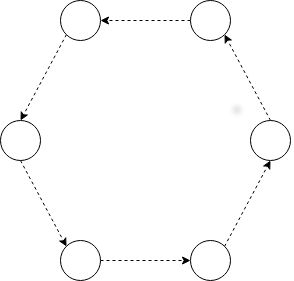
\includegraphics[width=.6\linewidth]{images/tcp}
  \caption{TCP Around Ring}
  \label{fig:tcp}
\end{subfigure}%
\begin{subfigure}{.5\textwidth}
  \centering
  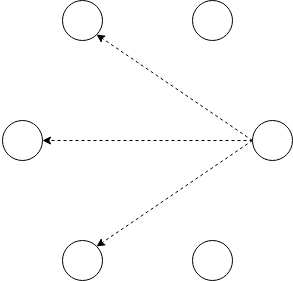
\includegraphics[width=.6\linewidth]{images/udp}
  \caption{UDP Across Ring}
  \label{fig:udp}
\end{subfigure}
\caption{The different types of communication used}
\label{fig:pattern}
\end{figure}

\section{Ring Formation}

\subsection{Initialization}

On initialization, each node sends out join messages to the coordinator. The
joining protocol is similiar to that described in \cite{join}, and is shown in Figure \ref{fig:join}.
Figure \ref{fig:bigjoin} shows how the state of each connection changes over the course of
the joining procedure.

\begin{figure}[!ht]
\centering
  \centering
  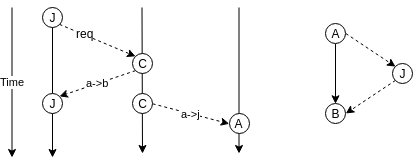
\includegraphics[width=.6\linewidth]{images/join}
  \caption{Joining protocol over time, with topology shown on right.}
\label{fig:join}
\end{figure}

\begin{figure}[!ht]
  \centering
  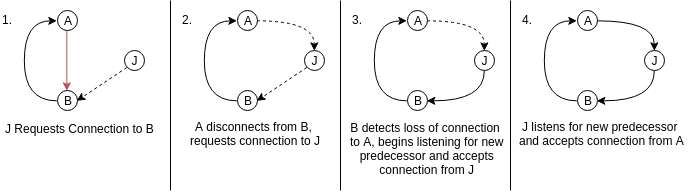
\includegraphics[width=\linewidth]{images/bigflow}
  \caption{State of each connection as a new node joins the ring. The red arrow
shows the edge that is replaced with the new node, and solid and dashed
arrows represent ongoing and pending connections respectively. Either A or
B can be the coordinator in this scenario.}
\label{fig:bigjoin}
\end{figure}
\FloatBarrier

\noindent When node J wants to join the ring:
\begin{enumerate}
    \item J sends join request to coordinator C.
    \item C sends successor to J, telling it to connect to B.
    \item C sends successor to A, telling it to connect to J. 
    \item A disconnects from B, B begins listening for new predecessor.
    \item J connects to B, A connects to J.
\end{enumerate}

In order for this process to work for a ring network with a single node,
it required another thread to wait on the connection, and the main thread
would then request the connection to itself. For two nodes and more the
joining node would be able to first connect to its new successor once its
predecessor had disconnected from its old successor as shown in figure \ref{fig:bigjoin}. 

\subsection{General Node Recovery}

When designing a distributed system, it should be assumed that failure will occur, and so as an extension this implementation included a mechanism for recovering from failure. Node failure is detected by either:
\begin{enumerate}
	\item a node attempting to read the socket connected to its predecessor.
	\item a node forwarding the token to its successor and not receiving an acknowledgement within a given timeframe.
\end{enumerate}

When a failure is detected by the successor of a failing node, it will simply begin listening for a new predecessor. Once the predecessor of the failing node detects the loss of connection, it will request a new successor from the coordinator node. The coordinator will then reply with the ID of the node after the failed node for the original predeccessor to connect to, at which point normal network behaviour can resume. Figure \ref{fig:failure} shows the topology change when a node fails.

\begin{figure}[!ht]
	\centering
	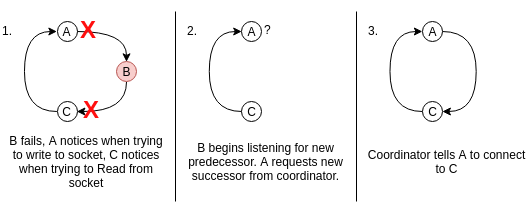
\includegraphics[width=\linewidth]{images/failure}
	\caption{Network topology during the recovery from node B failing. Either A or C are the coordinator in this scenario.}
	\label{fig:failure}
\end{figure}

The token acknowledgement message is the only occurence of communication in the reverse direction of the ring topology. The predecessor of the failing node will hold onto the token until it is assigned a new successor, and only releases the token once it has received the acknowlegement from it. This limits the number of situtations that can result in the loss of the token. If somehow the token is acknowledged but the message does not reach the predecessor in time, it could be possible for two tokens to then be in circulation. %TODO was this addressed?

\section{Leader/Coordinator Election}

% TODO LIMITATION: Cant have multiple nodes start up at the same time since node assumes itself coordinator

\section{Receive/Send Posts}

\bibliographystyle{unsrt}
\bibliography{mybib}

\end{document}
